\chapter{Additional Material for Chapter 5}
\graphicspath{{figures/ch_5/}}
\addtocontents{toc}{\protect\setcounter{tocdepth}{0}}

\section{Simulation model}
\label{ch_5:sec:full_simulation_model_explanation}
\addtocontents{toc}{\protect\setcounter{tocdepth}{2}}

\section{Additional Figures}

\begin{figure}
    \centering
    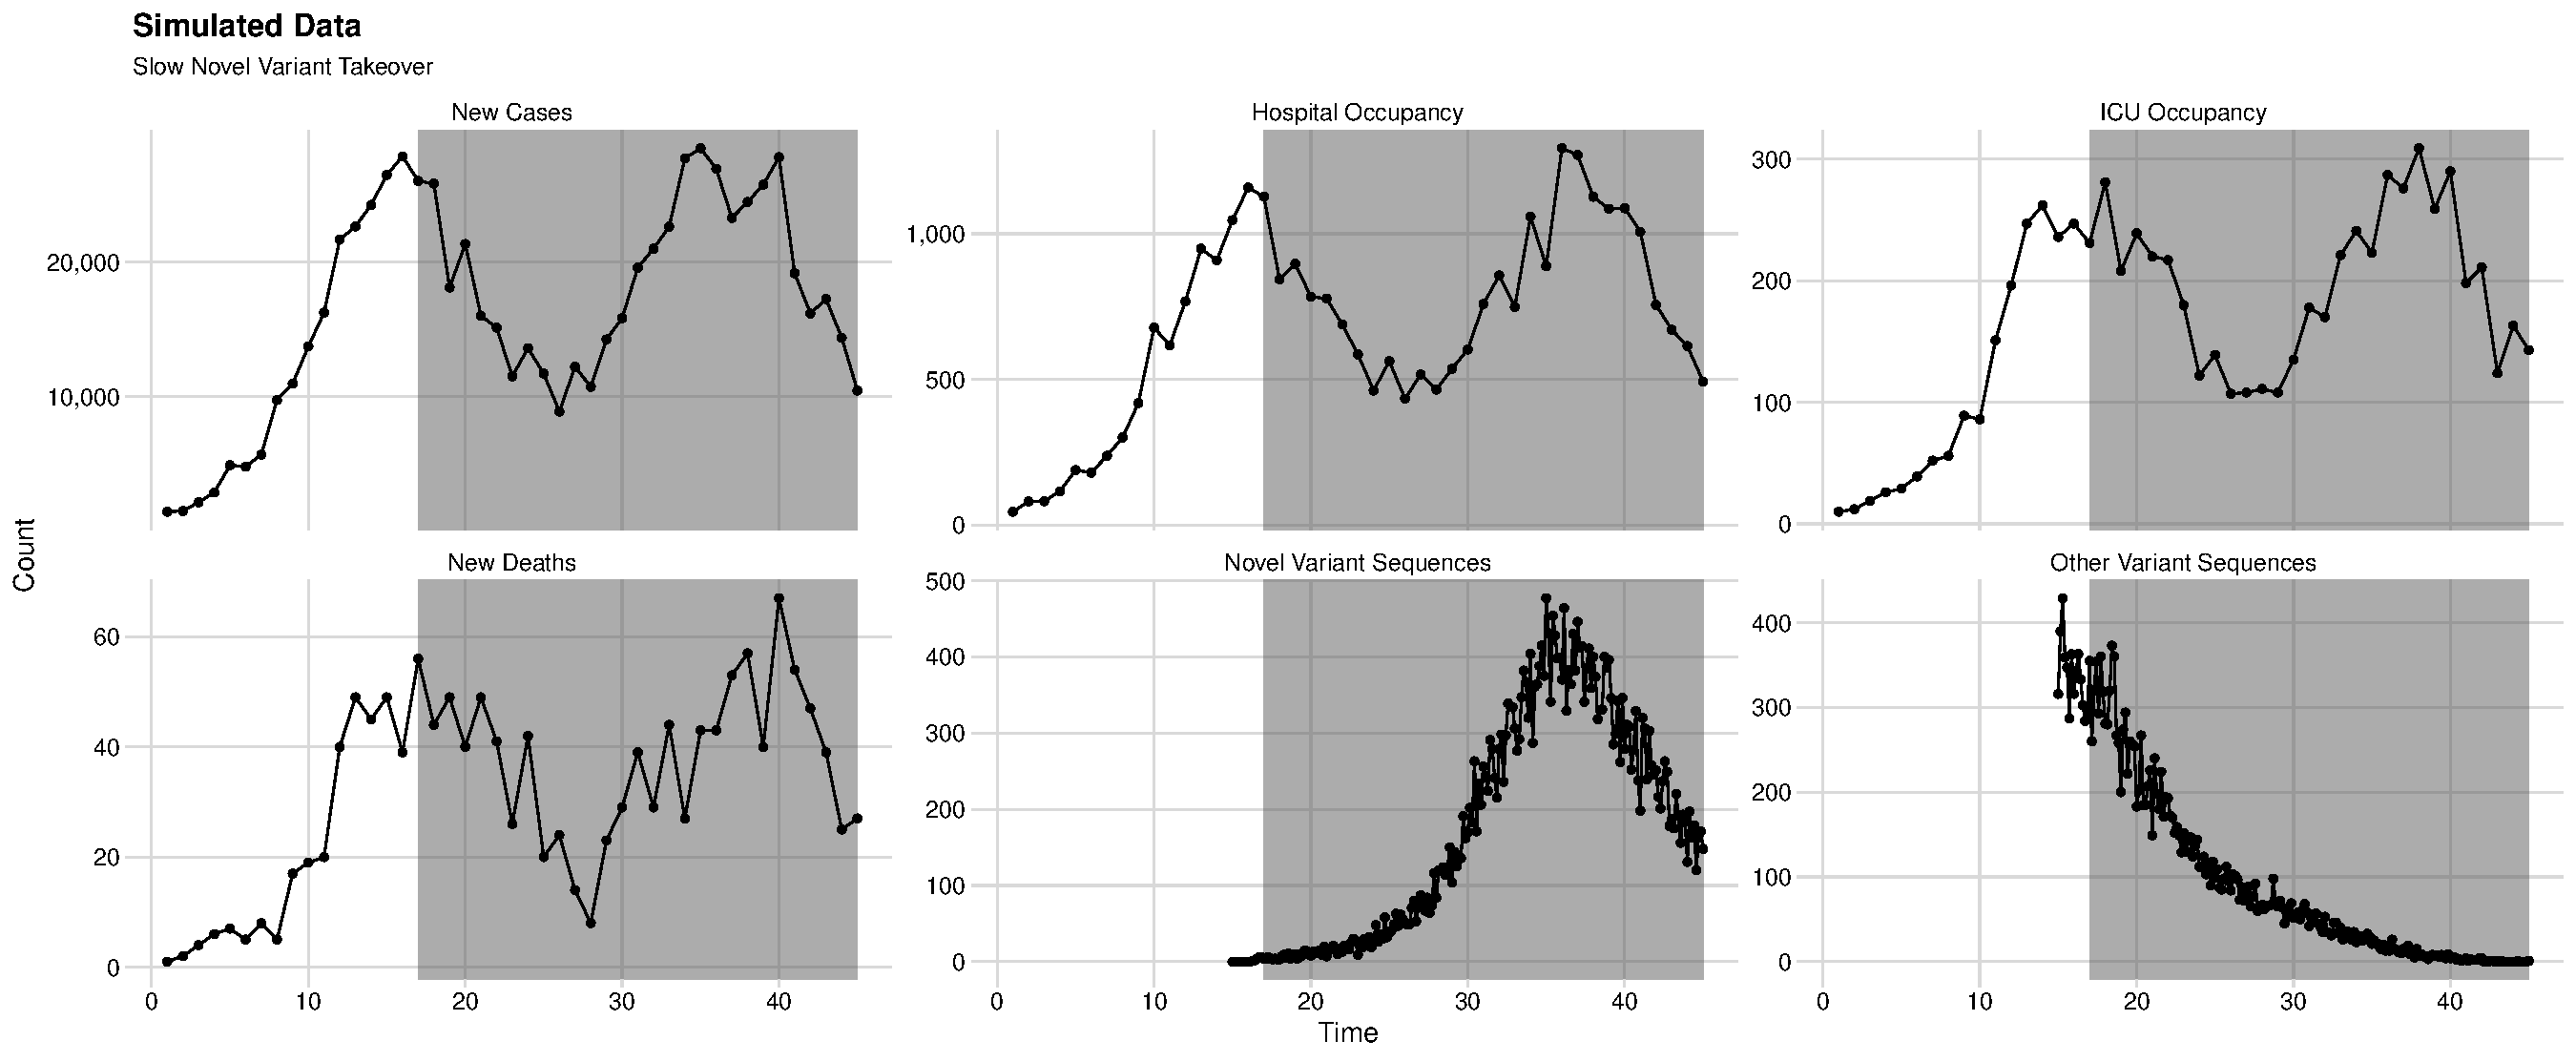
\includegraphics[width=1.0\columnwidth]{simulated_binned_data_slow_plot}
    \caption[Simulated data set for slow takeover speed scenario.]{Simulated data set for slow takeover speed scenario.
    The gray shaded areas indicating the time points for which we create forecasts}
    \label{ch_5:fig:simulated_binned_data_slow_plot}
\end{figure}

\begin{figure}
    \centering
    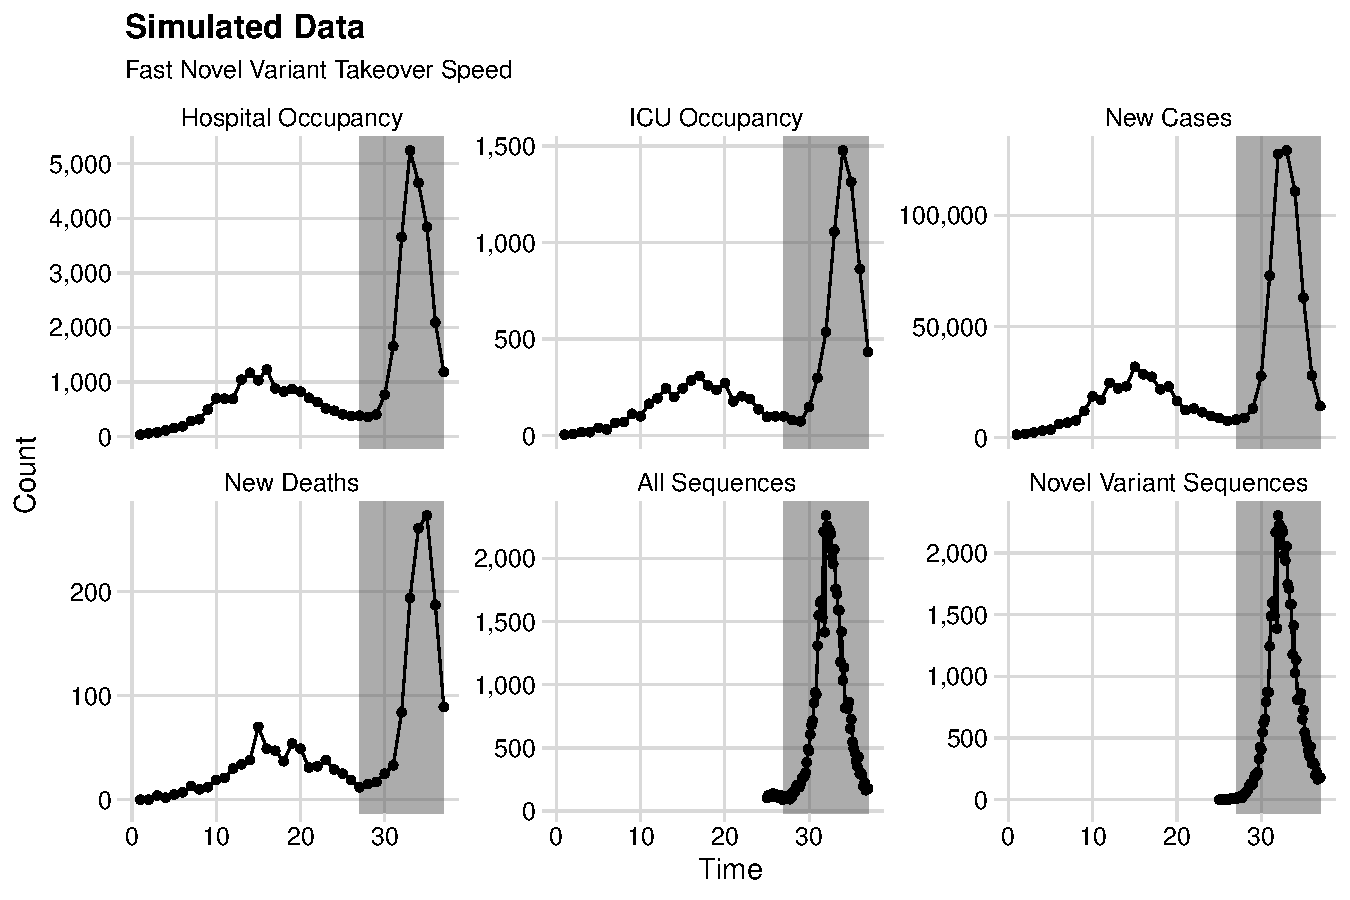
\includegraphics[width=1.0\columnwidth]{simulated_binned_data_fast_plot}
    \caption[Simulated data set for fast takeover speed scenario.]{Simulated data set for fast takeover speed scenario.
    The gray shaded areas indicating the time points for which we create forecasts}
    \label{ch_5:fig:simulated_binned_data_fast_plot}
\end{figure}

\section{Additional simulation study results for cases, ICU occupancy, and deaths}
\label{ch_5:sec:sim_cases_icu_death}

\begin{figure}
    \centering
    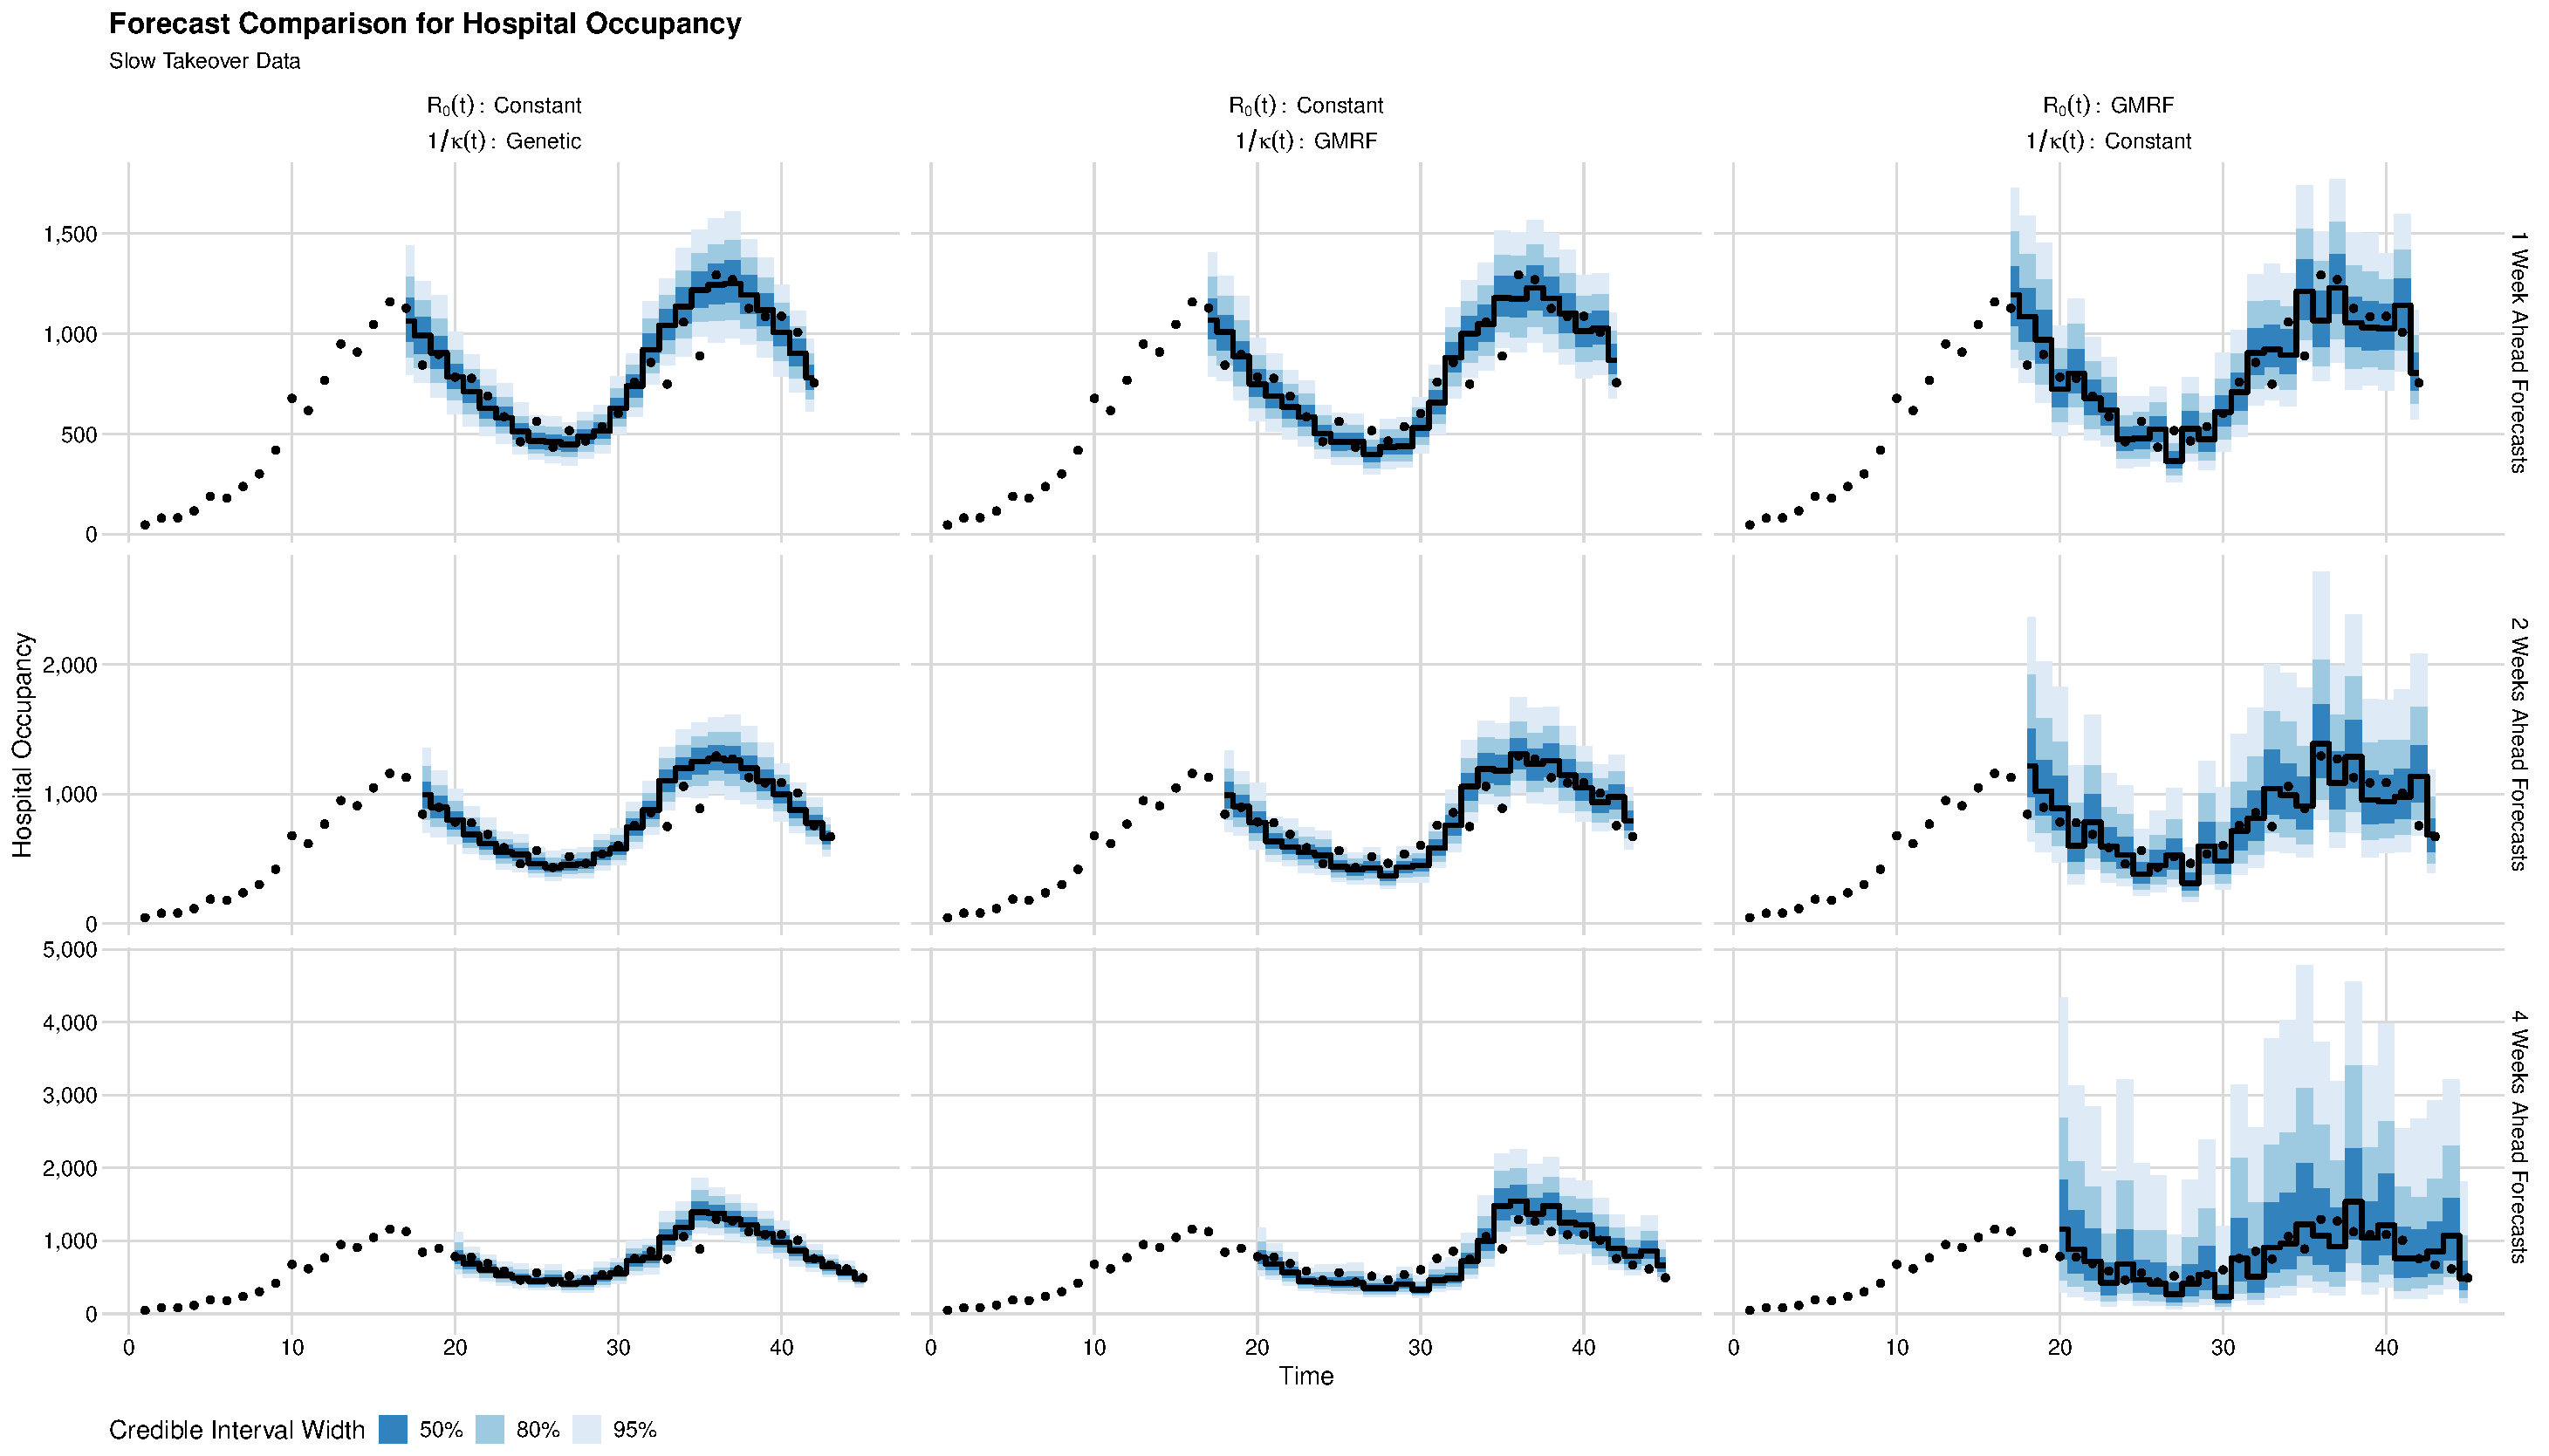
\includegraphics[width=1.0\columnwidth]{simulated_forecast_comparison_data_hospitalizations_slow_plot}
    \caption{Forecast from three models at 1, 2, and 4-week forecast horizons for the simulated slow takeover speed data.}
    \label{ch_5:fig:simulated_forecast_comparison_data_hospitalizations_slow_plot}
\end{figure}

\begin{figure}
    \centering
    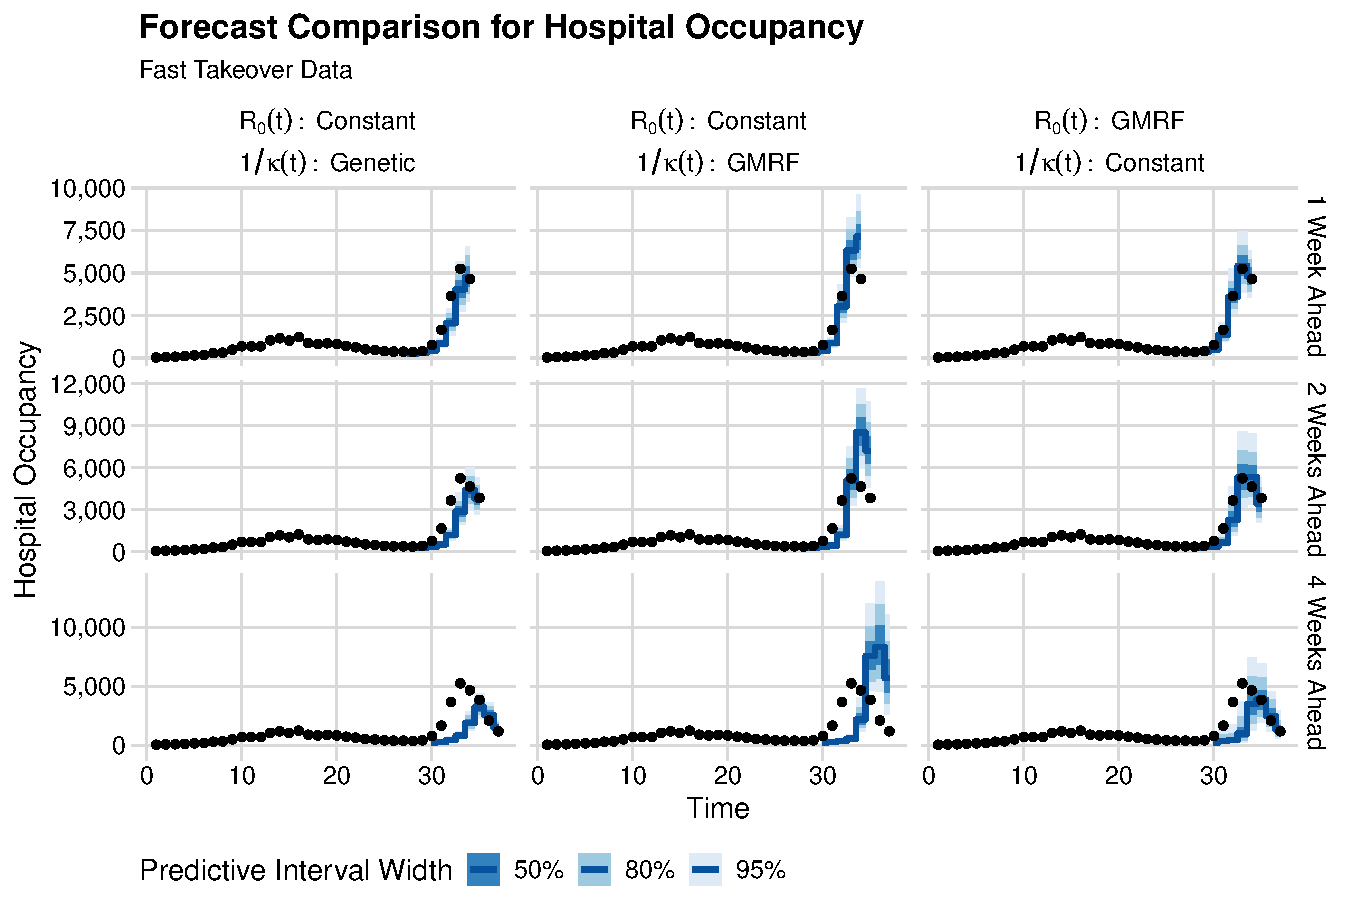
\includegraphics[width=1.0\columnwidth]{simulated_forecast_comparison_data_hospitalizations_fast_plot}
    \caption{Forecast from three models at 1, 2, and 4-week forecast horizons for the simulated fast takeover speed data.}
    \label{ch_5:fig:simulated_forecast_comparison_data_hospitalizations_fast_plot}
\end{figure}

\section{Simulation study sensitivity analysis}
\label{ch_5:sec:sim_sensitivity}